\newpage
\subsection{Quadratische Funktionen}

\begin{itemize}
    \item Die Grundform ist $y=a(x+b)^2+c$
    \item Faktorisierte Form ist $f(x)=a(x+x_1)*(x-x_2)$
    \item Scheitelpunktform oder Scheitelform ist $f(x)=a(x-d)^2+e$ mit Scheitel $S(d|e)$
\end{itemize}

\hfill \break
Veränderung der Normparabel:
\begin{itemize}
    \item Normparabel: \textcolor{black}{$x^2$}
    \item ist \textcolor{red}{$a<0$} wird die Funktion an der x Achse gespiegelt.
    \item ist \textcolor{blue}{$0<a<1$} wird die Funktion breiter bezihungsweise gestaucht.
    \item ist \textcolor{violet}{$a>1$} wird die Funktion steiler.
    \item ist \textcolor{cyan}{$x>0$} wird die Funktion nach oben verschoben.
    \item ist \textcolor{orange}{$x<0$} wird die Funktion nach oben verschoben.
    \item ist \textcolor{green}{$y<0$} wird die Funktion nach rechts verschoben.
    \item ist \textcolor{brown}{$y>0$} wird die Funktion nach links verschoben.
\end{itemize}

\hfill \break
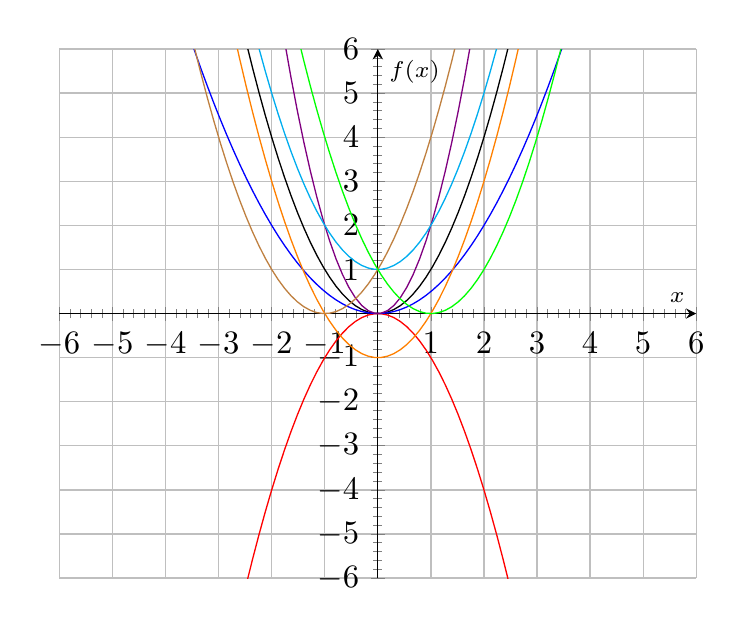
\begin{tikzpicture}[scale=1.18]
    \begin{axis}%
        [
            grid=major,
            xtick={-7,-6,...,7},
            minor x tick num=4, % 4 minor ticks => 5 subintervals
            xmin=-6,
            xmax=6,
            xlabel={\scriptsize $x$},
            axis x line=middle,
            ytick={-7,-6,...,7},
            minor y tick num=4,  % 4 minor ticks => 5 subintervals
            ymin=-6,
            ymax=6,
            ylabel={\scriptsize $f(x)$},
            axis y line=middle,
            no markers,
            samples=100,
            domain=-6:6,
        ]
        \addplot[black] (x,{x^2});
        \addplot[red] (x,{-1*x^2});
        \addplot[blue] (x,{0.5*x^2});
        \addplot[violet] (x,{2*x^2});
        \addplot[cyan] (x,{x^2+1});
        \addplot[orange] (x,{x^2-1});
        \addplot[brown] (x,{(x+1)^2});
        \addplot[green] (x,{(x-1)^2});
    \end{axis}
\end{tikzpicture}